\section{Network and data modeling}

\begin{frame}
  \frametitle{References}

    \begin{thebibliography}{99}
      \setbeamertemplate{bibliography item}[book]

    \bibitem[JW]{JW} Graphical Models in Applied Multivariate Statistics, \textcolor{black}{Joe Whittaker}
    \bibitem[SL]{SL} Graphical Models, \textcolor{black}{S. Lauritzen}
    \end{thebibliography}

\end{frame}

\subsection{Statistical dependence}

\begin{frame}
  \frametitle{Modeling relationship between variables}
  \framesubtitle{Independence}

  \begin{definition}[Independence of events]
    Two events $A$ and $B$ are independent if and only if
    \begin{equation*}
      \prob(A,B) = \prob(A) \prob(B),
    \end{equation*}
    which is usually denoted by $A \indep B$. Equivalently,
    \begin{itemize}
    \item $A \indep B \Leftrightarrow \prob(A | B) = \prob(A)$,
    \item $A \indep B \Leftrightarrow \prob(A | B) = \prob(A | B^c) $
    \end{itemize}
  \end{definition}

  \begin{example}[class vs party]<2>
    \vspace{-.5cm}
    \begin{table}
      \centering
      \begin{small}
      \begin{tabular}{cc}
        \begin{tabular}{rrr}
        & \multicolumn{2}{c}{party} \\
        class & Labour & Tory \\ \hline
        working & 0.42 & 0.28 \\
        bourgeoisie & 0.06 & 0.24 \\
      \end{tabular} 
      & 
      \begin{tabular}{rrr}
        & \multicolumn{2}{c}{party} \\
        class & Labour & Tory \\ \hline
        working & 0.60 & 0.40 \\
        bourgeoisie & 0.20 & 0.80 \\
      \end{tabular} 
      \end{tabular} 
      \caption{Joint probability (left) vs. conditional probability (right)} 
      \end{small}
    \end{table}
  \end{example}
\end{frame}

\begin{frame}
  \frametitle{Limits of correlation for network reconstruction}
  
  \includegraphics<1>[width=.65\textwidth]{cor_plot}

  \includegraphics<2>[width=.65\textwidth]{pcor_plot}
  
\end{frame}

\begin{frame}
  \frametitle{Modeling relationships between variables (2)}
  \framesubtitle{Conditional independence}
  
  Generalizing  to more  than two  events requires  strong assumptions
  (mutual independence). Better handle with

  \begin{definition}[Conditional independence of events]
    Two events $A$ and $B$ are conditionally independent if and only if
    \begin{equation*}
      \prob(A,B | C) = \prob(A|C) \prob(B|C),
    \end{equation*}
    which is usually denoted by $A \indep B | C$ 
  \end{definition}

  \begin{example}[Does QI depends on weight?]
    Consider  the  events $A  =  "\text{having low  QI}"$,  $B  = \text{"having  low
    weight"}$. \only<3>{Estimating\footnote{stupidly}  $\prob(A,B)$,  $\prob(A)$  and
    $\prob(B)$ in a sample would lead to
    \begin{equation*}
      \prob(A,B) \neq \prob(A) \prob(B)
    \end{equation*}}
  \only<4>{But in fact, introducing $C = \text{"having a given age"}$,
    \begin{equation*}
      \prob(A,B|C) = \prob(A|C) \prob(B|C)
    \end{equation*}}
\end{example}
  
\end{frame}

\begin{frame}
  \frametitle{(Conditional) independence of random vectors}
  \framesubtitle{A ``natural'' generalization}

   \begin{definition}   Consider   3   random   variables   $X,Y,Z$   with
     distribution $f_X,f_Y,f_Z$, jointly $f_{XY}, f_{XYZ}$. Then,
     \begin{itemize}
     \item  $X$  and $Y$  are  independent  iif  $f_{XY}(x,y) =  f_{X}(x)
       f_{Y}(y)$;
     \item $X$ and $Y$ are conditionally independent on $Z$, $z:f_Z(z)>0$ iif
       $f_{XY|Z}(x,y;z) = f_{X|Z}(x;z) f_{Y|Z}(y;z)$.
     \end{itemize}
   \end{definition}


   \def\firstcircle{(0,0) circle (2.25cm)}
   \def\secondcircle{(45:3.5cm) circle (2.25cm)}
   \def\thirdcircle{(0:3.5cm) circle (2.25cm)}

   % Now we can draw the sets:
   \begin{figure}[htbp!]
     \centering
     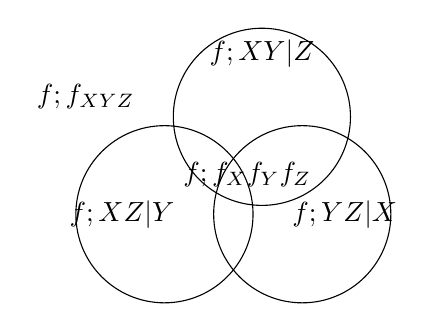
\begin{tikzpicture}[scale=.5]
     \draw \firstcircle node[left= -.25cm] {$f; X\indep Z | Y$};
     \draw \secondcircle node [above=.5cm] {$f; X\indep Y | Z$};
     \draw \thirdcircle node [right=-.25cm] {$f; Y\indep Z | X$};
     \draw (-2,3) node {$f; f_{XYZ}$};
     \draw (2.1,1) node {$f; f_{X} f_{Y} f_{Z}$};
   \end{tikzpicture}
     \caption{Mutual independence, Conditional dependence, full dependence.}
   \end{figure}

 \end{frame}

\subsection{Gaussian Graphical models}

\begin{frame}
  \frametitle{Graphical models}
  \begin{block}{Definition}
    A graphical model gives  a graphical (intuitive) representation of
    the dependence structure of a probability distribution, by linking
    
    \begin{enumerate}
    \item a random  vector (or a set of random  variables.)  $X = \{X_1,
      \dots, X_p\}$ with distribution $\prob$, \bigskip
    \item a graph $\mathcal{G} = (\mathcal{P}, \mathcal{E})$ where
      \begin{itemize}
      \item $\mathcal{P}=\{1,\dots,p\}$ is  the set of nodes associated
        to each variable,
      \item $\mathcal{E}$ is a  set of edges describing the dependence
        relationship of $X\sim \prob$.
      \end{itemize}
    \end{enumerate}
   \end{block}

   \vfill

  \begin{definition}<2> The  \alert{conditional independence graph}  of a
    random vector  $X$ is the \alert{undirected}  graph $\mathcal{G} =
    \{\mathcal{P},    \mathcal{E}\}$   with    the    set   of    node
    $\mathcal{P}=\{1,\dots,p\}$ and where
    \begin{equation*}
      (i,j) \notin \mathcal{E} \Leftrightarrow X_i \indep X_j | \mathcal{P} \backslash
      \{i,j\}.
    \end{equation*}
  \end{definition}

\end{frame}

\begin{frame}
  \frametitle{Conditional Independence Graphs}
  \framesubtitle{An example}
  
  Let  $X_1,  X_2, X_3,  X_4$  be  four  random variables  with  joint
  probability density  function $f_X(x) =  \exp(u + x_1+x_1 x_2  + x_2
  x_3 x_4)$ with $u$ a given constant.
  
  \begin{block}{Apply the factorization property}
    \begin{equation*}
      \begin{aligned}
        f_X(x) & = \exp(u + x_1+x_1 x_2 + x_2 x_3 x_4) \\
        &  = \exp(u)\  \cdot \  \alert<3>{\exp(x_1+x_1 x_2)}\  \cdot \
        \alert<4>{\exp(x_2 x_3 x_4)} 
      \end{aligned}
    \end{equation*}
  \end{block}
  
  \vfill

  \begin{block}{Graphical representation}<2->
    
    \begin{columns}[c]
      \begin{column}{.5\textwidth}
        $\mathcal{G} = (\mathcal{P},\mathcal{E})$ such as $\mathcal{P}
        = \{1,2,3,4\}$ and 
        \begin{equation*}
          \mathcal{E} = \only<2>{\{?\}}
          \only<3>{\{(1,2)\}}
          \only<4->{\{(2,3),(3,4),(2,4)\}}
        \end{equation*}
      \end{column}
      \begin{column}{.5\textwidth}
        \begin{center}
          \begin{tikzpicture}
            \node[state] (1) at (0,0) {1}; 
            \node[state] (2) at (2,0) {2}; 
            \node[state] (3) at (3,-2) {3};
            \node[state] (4) at (4,0) {4};
            \onslide<3->{ \path (1) edge (2) ; }
            \onslide<4->{ \path (2) edge (3) (3) edge (4) (2) edge (4) ; }
          \end{tikzpicture}
        \end{center}
      \end{column}
    \end{columns}
  \end{block}

\end{frame}

\begin{frame}
  \frametitle{The Gaussian case}

  \begin{block}{The data}
    \begin{tikzpicture}
      \node[opacity=.75] at (-3,1.5) {\pgfuseimage{microarray}};
      \node[opacity=.9] at (-2.75,1.25) {\pgfuseimage{microarray}};
      \node[opacity=.95] at (-2.5,1) {\pgfuseimage{microarray}};
      \node at (-2.25,0.75) {\pgfuseimage{microarray}};
      \node[fill=red, text=white,single arrow] 
      (inference) at (0,1) {\sf \scriptsize Inference}; 
          
      \node at (4.5,1) {%
        $\mathbf{X} = \begin{pmatrix} 
          x_1^1 & x_1^2 & x_1^3 & \dots & x_1^p \\
          \vdots \\
          x_n^1 & x_n^2 & x_1^2 & \dots & x_n^p \\
        \end{pmatrix}$};
    \end{tikzpicture}
  \end{block}

  \begin{block}{Assuming $f_X(\mathbf{X})$ multivariate Gaussian}
    Greatly simplifies the inference:
    \begin{itemize}
    \item[$\rightsquigarrow$]   naturally   links   independence   and
      conditional   independence  to   the   covariance  and   partial
      covariance,
    \item[$\rightsquigarrow$]  gives a  straightforward interpretation
      to the graphical modeling previously considered.
  \end{itemize}
  \end{block}
\end{frame}


\begin{frame}
  \frametitle{Why Gaussianity helps?}
  \framesubtitle{Case of 2 variables or size-2 random vector}

  \begin{definitions}[Let $X,Y$ be two real random variables.]
    \vspace{-.75cm}
    \begin{equation*}
      \cov(X,Y)   =  \E\Big[\big(X-\E(X)\big)\big(Y-\E(Y)\big)\Big]  =
      \E(XY) - \E(X)\E(Y).
    \end{equation*}
    \begin{equation*}
      \rho_{XY} = \cor(X,Y) = \frac{\cov(X,Y)}{\sqrt{\var(X) \ \cdot \ \var(Y)}}.
    \end{equation*}
  \end{definitions}
  
  \begin{proposition}
    \begin{itemize}
    \item $\cov(X,X) = \var(X) = \E[(X-\E X)(Y-\E Y)]$,
    \item $\cov(X+Y,Z) = \cov(X,Z) + \cov(X,Z)$,
    \item $\var(X+Y) = \var(X) + \var(Y) + \cov(X,Y)$.
    \item $X \indep Y \Rightarrow\cov(X,Y) = 0$.
    \item<2> \alert{$X  \indep Y  \Leftrightarrow \cov(X,Y) =  0$ when
        $X,Y$ are Gaussian}.
    \end{itemize}
  \end{proposition}
\end{frame}

\begin{frame}
  \frametitle{The bivariate Gaussian distribution}

  \begin{columns}
    \begin{column}{.4\textwidth}
      \begin{block}{The Covariance Matrix}
        Let
        \begin{equation*}
          X \sim \mathcal{N}(\mathbf{0}, \boldsymbol\Sigma), 
        \end{equation*}
        with unit variance and $\rho_{XY} = \only<1>{0}\only<2>{0.9}$
        \begin{equation*}
          \boldsymbol\Sigma =
          \begin{pmatrix}
            1 & \only<1>{0}\only<2>{0.9} \\ \only<1>{0}\only<2>{0.9} & 1
          \end{pmatrix}.
        \end{equation*}
        The shape of the 2-D distribution evolves accordingly.
      \end{block}
    \end{column}
    
    \begin{column}{.6\textwidth}
      \includegraphics<1>[height=.8\textheight]{figures/multinorm_nocor}
      \includegraphics<2>[height=.8\textheight]{figures/multinorm_cor}
    \end{column}
  \end{columns}
\end{frame}

\begin{frame}
  \frametitle{Generalization: multivariate Gaussian vector}
  \framesubtitle{Now need partial covariance and partial correlation}
  
  Let $X,Y,Z$ be real random variables.
  \begin{definitions}
    \begin{equation*}
      \cov(X,Y|Z) = \cov(X,Y) - \cov(X,Z)\cov(Y,Z)/\var(Z).
    \end{equation*}
    \begin{equation*}
      \rho_{XY|Z}            =            \frac{\rho_{XY}            -
        \rho_{XZ}\rho_{YZ}}{\sqrt{1-\rho_{XZ}^2}\sqrt{1-\rho_{YZ}^2}}.
    \end{equation*}
  \end{definitions}
  $\rightsquigarrow$  Give   the  interaction  between   $X$  and  $Y$
  \alert{once removed the effect of $Z$}.

  \vfill
  
  \begin{proposition}<2>
    When $X,Y,Z$ are jointly Gaussian, then
    \begin{equation*}
      \alert{\cov(X,Y|Z) = 0  \Leftrightarrow \cor(X,Y|Z) = 0 \Leftrightarrow
      X \indep Y | Z.}
    \end{equation*}
  \end{proposition}
\end{frame}


\begin{frame}
  \frametitle{Gaussian Graphical Model: canonical settings}

  \begin{block}{Experiments in comparable Gaussian conditions}
    \begin{enumerate}
    \item  $X\sim\mathcal{N}(\boldsymbol\mu,\boldsymbol\Sigma)$,  with
      $\boldsymbol\Omega = \bSigma^{-1}$ the precision matrix.
    \item a sample $(X^1, \dots, X^n)$ of exp. stacked in an $n\times
      p$ data matrix $\mathbf{X}$.
    \end{enumerate}
  \end{block}

  \vspace{-.5cm}

  \begin{overlayarea}{\textwidth}{\textheight}
    \begin{block}{Conditional independence structure}
          \vspace{-.5cm}
          \begin{equation*}
            (i,j)  \notin  \mathcal{E}  \Leftrightarrow  X_i  \indep  X_j  |
            X_{\backslash \{i,j\}} \Leftrightarrow \Omega_{ij} = 0.
          \end{equation*}
        \end{block}
        
        \vspace{-.5cm}
        \begin{block}{Graphical interpretation}
          \vspace{-.5cm}
          \begin{center}
            \begin{tabular}{c@{\hspace{2cm}}c}
              \begin{tabular}{c}
                \small $\mathcal{G}=(\mathcal{P},\mathcal{E})$ \\
                \includegraphics[width=.3\textwidth]{graph}
              \end{tabular}
              &
              \begin{tabular}{c}
                \small $\bTheta$\\\includegraphics[width=.2\textwidth]{Markovadjacency}
              \end{tabular}
            \end{tabular}
          \end{center}
        \end{block}
        \vspace{-1cm}
        $\rightsquigarrow$ \alert{``Covariance'' selection}
   
  \end{overlayarea}      
\end{frame}

\begin{frame}
  \frametitle{Gaussian vector and linear regression (I)}

  \begin{proposition}[Gaussian vector and conditioning]
    \begin{equation*}
      Z = \begin{pmatrix}
        Z_1 \\ Z_2
      \end{pmatrix}  \sim   \mathcal{N}(\mathbf{0},\bSigma),   \quad
      \bSigma = \begin{pmatrix}
        \bSigma_{11} & \bSigma_{12} \\
        \bSigma_{21} & \bSigma_{22} \\
      \end{pmatrix},\quad
      \bOmega = \bSigma^{-1} = \begin{pmatrix}
        \bOmega_{11} & \bOmega_{12} \\
        \bOmega_{21} & \bOmega_{22} \\
      \end{pmatrix}.
    \end{equation*}
    Then,
    \begin{equation*}
      Z_2|Z_1=\mathbf{z} \sim
      \mathcal{N}\left(-\bOmega_{22}^{-1}\bOmega_{21}\mathbf{z}, \bOmega_{22}^{-1} \right)
    \end{equation*}
    and
    \begin{equation*}
      \bOmega_{22}^{-1}     =      \bSigma_{22}     -     \bSigma_{21}
      \bSigma_{11}^{-1} \bSigma_{12}.
    \end{equation*}
  \end{proposition}

  \vfill

  \begin{block}{Corollary}
    Partial correlations are related  to the inverse of the covariance
    matrix:
    \begin{equation*}
      \cor(Z_i,Z_j|Z_k, k\neq i,j) = - \frac{\Omega_{ij}}{\sqrt{\Omega_{ii}\Omega_{jj}}}
  \end{equation*}
  \end{block}

\end{frame}

\begin{frame}
  \frametitle{Gaussian vector and linear regression (II)}

  Consider the linear model
  \begin{equation}
      \label{eq:usual_lm}
    Y = X^\intercal\bbeta + \varepsilon, \quad \varepsilon\sim\mathcal{N}(0,\sigma).
  \end{equation}

  \begin{overlayarea}{\textwidth}{\textheight}

    \begin{block}{Other interpretation for the regression coefficients}
      If   $(X^T,  Y)^T\sim   \mathcal{N}(\mathbf{0},\bSigma)$  with   a
      block-wise  decomposion  of $\bSigma$  and  $\bOmega=\bSigma^{-1}$
      then by condition $Y|X$ we get
      \begin{equation}
        \label{eq:partial_lm}
        Y      =    \sum_{j=1}^p  X_j     \cor(X_j,Y|X_k,      k\neq      j)
        \sqrt{\frac{(\bOmega_{XX})_{jj}}{\omega_{YY}}}+ \varepsilon,
        \quad \varepsilon\sim\mathcal{N}(0,1/\omega_{YY}).
      \end{equation}

      By comparing \eqref{eq:usual_lm} to \eqref{eq:partial_lm}
      then \alert{$\beta_j$ is related to the partial correlation between $X_j$
        and $Y$},  i.e. describes  effect of  $X_j$ on  $Y$ once  effect of
      other predictors have been removed.
    \end{block}

  \end{overlayarea}
\end{frame}

\begin{frame}
  \frametitle{Gaussian Graphical Model and Linear Regression}

  \begin{block}{Linear regression viewpoint}
    Variable $X_i$ is linearly explained by the other variables:
    \begin{equation*}
      X_i | X_{ \setminus i} = - \sum_{j \neq i}
      \frac{\Theta_{ij}}{\Theta_{ii}} X_j + \varepsilon_i,\quad \varepsilon_i
      \sim \mathcal{N}(0,\sigma_i), \quad \varepsilon_i \perp X
      \end{equation*}
      Conditional  on its  neighborhood,  other variables do not  give
      additional insights
    \begin{equation*}
      X_i | X_{ \setminus i} = \sum_{\alert{j \in \text{neighbors}(i)}} \beta_j X_j + \varepsilon_i
      \quad         \text{with         }         \beta_j         =
      -\frac{\Theta_{ij}}{\Theta_{ii}}.
    \end{equation*}
  \end{block}

  % \vspace{-.5cm}
  % \begin{overlayarea}{\textwidth}{.45\textheight}
  %   \begin{block}{Graphical Interpretation}
  %     \vspace{-.5cm}
  %     \begin{center}
  %       \begin{scriptsize}
  %         \begin{tabular}{cc}
  %           Local Markov property & Global Markov property \\
  %           conditioning on the neighborhood & conditioning on a separating node\\
  %           \includegraphics[width=.4\textwidth]{localMarkov}
  %           & \includegraphics[width=.4\textwidth]{globalMarkov}\\
  %         \end{tabular}
  %       \end{scriptsize}
  %     \end{center}
  %   \end{block}
  % \end{overlayarea}

  \vfill
  \alert{$\rightsquigarrow$ ``Neighborhood'' selection}

\end{frame}
